\section{Methods and Materials}

\subsection{ANTs volumetric-based cortical thickness estimation pipeline}

The ANTs-based cortical thickness estimation workflow is illustrated 
in Figure \ref{fig:pipeline}.  The steps are as follows:
\begin{enumerate}
  \item initial N4 bias correction on input anatomical MRI,
  \item brain extraction using a hybrid segmentation/template-based strategy,
  \item alternation between prior-based segmentation and ``pure tissue'' 
        posterior probability weighted bias correction,
  \item DiReCT-based cortical thickness estimation, and
  \item optional normalization to specified template.
\end{enumerate}
Each component, including both software and data, is briefly detailed 
below with the relevant references for additional information. 

%We also note that each component is publicly available with all ANTs 
%algorithms available as open source.%
%\footnote{
%http://www.picsl.upenn.edu/ANTS
%}
The coordination of all the algorithmic components is
encapsulated in the shell script \verb#antsCorticalThickness.sh# with
subcomponents delegated to \verb#antsBrainExtraction.sh# 
and \verb#antsAtroposN4.sh#.  Extensive tuning produced
optimal parameters for processing the data sets
described in this work and should be extendable to 
other data sets.

%\lstset{frame = tb,
%        framerule = 0.25pt,
%        float,
%        fontadjust,
%        backgroundcolor={\color{listlightgray}},
%        basicstyle = {\ttfamily\scriptsize},
%        keywordstyle = {\ttfamily\color{listkeyword}\textbf},
%        identifierstyle = {\ttfamily},
%        commentstyle = {\ttfamily\color{listcomment}\textit},
%        stringstyle = {\ttfamily},
%        showstringspaces = false,
%        showtabs = false,
%        numbers = none,
%        numbersep = 6pt,
%        numberstyle={\ttfamily\color{listnumbers}},
%        tabsize = 2,
%        language=,
%        floatplacement=!h,
%        caption={\small \baselineskip 12pt DiReCT long command line menu which is invoked using the `{\ttfamily {-}{-}help}' option.  The short command line menu is obtained by typing `{\ttfamily {-}h}'}.,
%        captionpos=b,
%        label=listing:long
%        }
%\lstsetcpplong
%\begin{lstlisting}
%This script, apb.sh, performs T1 anatomical brain 
%processing where the following steps are currently 
%applied:
%
%  1. Brain extraction
%  2. Brain 3-tissue segmentation
%  3. Cortical thickness
%  4. (Optional) registration to a template
%
%Usage:
%
%abp.sh -d ImageDimension
%       -i T1Image.nii.gz
%       -e BrainExtractionTemplate
%       -m BrainExtractionProbabilityMask
%       -l BrainParcellationTemplate
%       -p BrainParcellationProbabilityMask
%       <OPTARGS>
%       -o OutputPrefix
%
%Example:
%
%abp.sh -d 3 
%       -i t1.nii.gz 
%       -e brainWithSkullTemplate.nii.gz 
%       -m brainPrior.nii.gz 
%       -l corticalLabels.nii.gz 
%       -p corticalLabelPriors.nii.gz 
%       -o output
%
%Compulsory arguments:
%
%     -d:  ImageDimension                        2 or 3 (for 2 or 3 dimensional single image)
%     -a:  Anatomical T1 image                   typically T1.
%     -e:  Brain extraction template             Anatomical template created using e.g. LPBA40 data set with
%                                                buildtemplateparallel.sh in ANTs.
%     -m:  Brain extraction probability mask     Brain probability mask created using e.g. LPBA40 data set which
%                                                have brain masks defined, and warped to anatomical template and
%                                                averaged resulting in a probability image.
%     -l   Brain segmentation template           Anatomical template for brain segmentation.  E.g. NIREP template
%                                                with labels.
%     -p   Brain segmentationpriors              Label probability priors corresponding to the image specified
%                                                with the -l option.  Specified using c-style formatting, e.g.
%                                                -p labelsPriors\%02d.nii.gz.
%     -o:  OutputPrefix                          The following images are created using the specified prefix:
%                                                  * /Users/ntustison/Data//tmp13243//tmpN4Corrected.nii.gz
%                                                  * /Users/ntustison/Data//tmp13243//tmpExtractedBrain.nii.gz
%                                                  * /Users/ntustison/Data//tmp13243//tmp3TissueBrainSegmentation.nii.gz
%                                                  * /Users/ntustison/Data//tmp13243//tmpCorticalThickness.nii.gz
%                                                  * /Users/ntustison/Data//tmp13243//tmpSurfaceCurvature.nii.gz
%
%Optional arguments:
%
%     -s:  image file suffix                     Any of the standard ITK IO formats e.g. nrrd, nii.gz (default), mhd
%     -t:  template for t1 registration
%     -k:  keep temporary files                  Keep brain extraction/segmentation warps, etc (default = false).
%     -w:  white matter label                    white matter label for segmentation (default = 3).
%     -g:  gray matter label                     cortical gray matter label for segmentation (default = 2)
%     -i:  max iterations for registration       ANTS registration max iterations (default = 50x100x20)
%\end{lstlisting}



\begin{figure*}
  \centering
  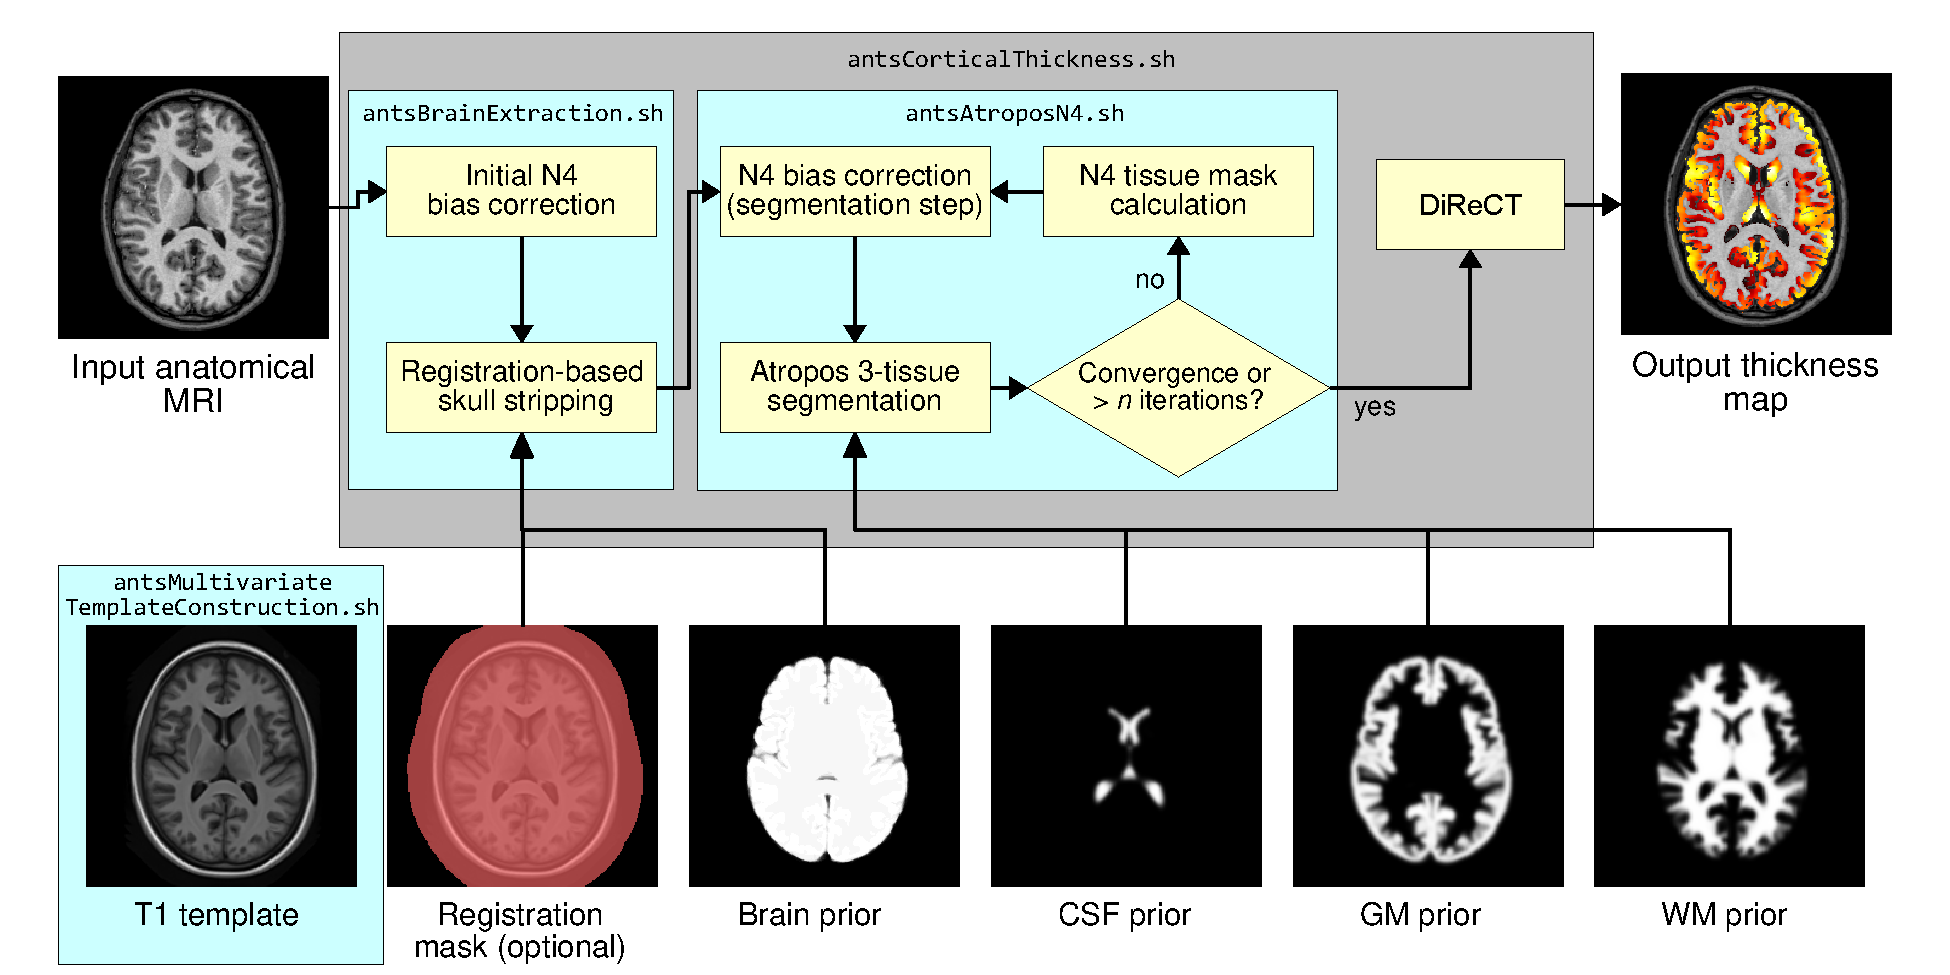
\includegraphics[width=140mm]{Figures/Kapowski_pipeline2.pdf}
  \caption{Illustration of the main components of the ANTs processing 
  workflow containing all elements for determining cortical thickness. 
  We also included the domain of operations for the selected scripts.
  Not shown is the optional subject to template registration.}
  \label{fig:pipeline}
\end{figure*}

\subsubsection{Anatomical template construction}

Normalizing images to a standard coordinate system
reduces intersubject variability in population studies.  Various
approaches exist for determining the normalized space such as the selection
of a pre-existing template based on a single subject, e.g. the Talairach
atlas \citep{Talairach1988}, or a publicly available averaged group of
subjects, e.g. the MNI \citep{Collins1994} or ICBM \citep{Mazziotta1995}
templates.  Additionally, mean templates constructed from labeled
data can be used to construct spatial priors for improving segmentation
algorithms.
The work of \cite{avants2010} explicitly models the geometric component of the 
normalized space during optimization to produce such mean templates.  Coupling the intrinsic symmetry of 
SyN pairwise registration \citep{avants2011} and an
optimized shape-based sharpening/averaging of the template appearance, Symmetric Group
Normalization (SyGN) is a powerful framework for producing optimal population-specific
templates.

%One challenge with standard templates is that they may inadvertently bias one's results by enabling better normalization of subjects to which the template is more similar.  This issue is exacerbated when dealing with populations that have high variance (e.g. due to disease) and/or when one's normalization method is low-dimensional (not flexible enough to capture large shape differences). 

%Population-specific templates alleviate some of
%the issues with other template approaches by deriving a most representative image from the population
%\citep{Good2001}.  Large deformation registration algorithms also reduce
%this confound by being less sensitive to the deformation distance
%between subject and target.  Some approaches combine both advantages,
%for instance, the diffeomorphic approach of Joshi et al. employs the
%SSD metric and a shape distance to bring the subject group of images
%into alignment \citep{Joshi2004}.  Variants
%include extension to multiple modalities \citep{Lorenzen2006} and small deformations
%\citep{Geng2009}.  These approaches iteratively minimize group difference in ``congealing''
%towards a representative image template \citep{Learned-Miller2006}.


The ANTs implementation of this technique is currently available as a shell script, 
\verb#buildtemplateparallel.sh#.  A generalized, multivariate version is also available as
\verb#antsMultivariateTemplateConstruction.sh#.  Both scripts are distributed as part of
 the ANTs repository.
The multivariate script permits the construction of multimodal templates (e.g. 
T1-weighted, T2-weighted, proton density MRI and fractional anisotropy).  
Both scripts accommodate a variety of computational resources
for facilitating template construction.  These computational resource possibilities include:
\begin{itemize}
  \item serial processing on a single workstation, 
  \item parallelized processing on a single workstation with multiple cores using \verb#pexec#%
  \footnote{http://www.gnu.org/software/pexec/pexec.1.html},
  \item parallelized processing using Apple's XGrid technology%
  \footnote{https://developer.apple.com/hardwaredrivers/hpc/xgrid\_intro.html}, 
  \item parallelized processing using Sun Grid Engine for cluster-based systems%
  \footnote{http://www.oracle.com/technetwork/oem/grid-engine-166852.html}, and 
  \item parallelized processing using the Portable Batch System for cluster-based systems%
  \footnote{http://www.pbsworks.com/}.
\end{itemize}

For this work, database-specific templates were used during cortical thickness pipeline
processing for both brain extraction and brain segmentation steps.  Multivariate templates 
were constructed from the multimodal data sets.  However, their usage was based on the 
fact that they had been built previously for other work and not because they provide a 
discernible advantage over univariate templates (i.e. T1-only) for the proposed workflow.

%Given a set of representative images, 
%$\{I_1, I_2, \ldots, I_M\}$, optimization involves finding the set of paired
%diffeomorphic transformations, $\left\{\left(\phi^1_1, \phi^1_2\right), 
%\left(\phi^2_1, \phi^2_2\right), \ldots, \left(\phi^M_1, \phi^M_2\right) \right\}$,
%the optimal template appearance, $J^*$, and corresponding coordinate system, $\psi(\mathbf{x})$,
%which minimize the following cost function:
%\begin{align}
%  \sum_{m=1}^M \left[
%    D\left( \psi(\mathbf{x}), \phi^m_1(\mathbf{x}, 1) \right) + 
%    \Pi \left( I_m\left(\phi^m_2(\mathbf{x}, 0.5) \right), J^*\left(\phi^m_1(\mathbf{x}, 0.5) \right) \right)
%    \right]
%\end{align}
%where $D$ is the diffeomorphic shape distance, 
%\begin{align}
%  D\left(\phi(\mathbf{x}, 0), \phi(\mathbf{x}, 1)\right) = \int_{0}^1 \| v(\mathbf{x}, t) \|_L dt, 
%\end{align}
%dependent upon the choice of the linear operator, $L$, and
%$v$ is the diffeomorphism-generating velocity field, 
%\begin{align}
%  v\left(\phi(\mathbf{x}, t), t \right) = \frac{d\phi(\mathbf{x}, t)}{dt},\,\,\, \phi(\mathbf{x}, 0) = \mathbf{x}.
%\end{align}
%$\Pi$ is th
%e choice of similarity metric, often cross-correlation \citep{Avants2008a}, calculated in the 
%virtual domain midway between each individual image and the current estimate of the template. 
%
%With initial assignment of $\left\{\left(\phi^m_1, \phi^m_2\right)\right\}$ and $\psi(\mathbf{x})$ 
%to identity, iterative optimization
%involves estimating the pairwise transformations, estimation of the optimal template appearance, and 
%updating $\psi(\mathbf{x})$ by averaging the current estimate of $\left\{\phi_1^m\right\}$.  


\subsubsection{N4 Bias field correction}

Critical to quantitative processing of MRI is the minimization of
field inhomogeneity effects which produce artificial low frequency 
intensity variation across the image.  Large-scale studies, such
as the Alzheimer's Disease Neuroimaging Initiative (ADNI), employ
perhaps the most widely used bias correction algorithm, N3 \citep{sled1998}, 
as part of their standard protocol \citep{boyes2008}.

In \cite{tustison2010}, we introduced an improvement of N3, denoted as
``N4'', which demonstrates a significant increase in performance and convergence behavior
on a variety of data.  This improvement is a result of an enhanced 
fitting routine (which includes multi-resolution capabilities) and a modified optimization 
formulation.  For our workflow, the additional possibility of specifying
a weighted mask in N4 permits the use of a ``pure tissue'' probability map 
(described below)
calculated during the segmentation pipeline for further improvement of 
bias field estimation.  In addition to its public availability 
through ANTs and the Insight Toolkit, it has also been included in
the popular open source Slicer software package for visualization and medical
image computing \citep{fedorov2011}.

N4 is used in two places during the individual subject processing (cf. Figure
\ref{fig:pipeline}).  Following conversion of the raw dicom T1-weighted image
to Nifti format using our related \verb#Neuropipedream# set of raw image conversion
and organization tools%
\footnote{
http://sourceforge.net/projects/neuropipedream/
}, N4 is used to generate an initial bias corrected image for use in
brain extraction.  The input mask is created by adaptively thresholding 
the background from the foreground using Otsu's algorithm \citep{otsu1979}.
Following brain extraction, three-tissue segmentation involves iterating
between bias field correction using the current pure tissue 
probability map as a weight mask and then using that bias corrected image
as input to the Atropos segmentation step (described in the next section). 

\subsubsection{Atropos 3-tissue segmentation}

In \cite{avants2011a} we presented an open source $n$-tissue segmentation software tool
(which we denote as ``Atropos'') attempting to distill 20+ years of active research in this area
particularly some of its most seminal work (e.g. \cite{zhang2001,ashburner2005}). 
Specification of prior probabilities includes spatially varying Markov Random Field modeling, 
prior label maps, and prior probability maps typically derived from our template building 
process.  Additional
capabilities include handling of multivariate data, 
partial volume modeling \citep{shattuck2001}, a memory-minimization mode,
label propagation, a plug-n-play architecture for incorporation of novel likelihood models
which includes both parametric and non-parametric models for both scalar and tensorial
images, and alternative posterior formulations for different segmentation tasks.

Due to the important interplay between segmentation and bias correction,
we perform multiple N4 $\rightleftharpoons$ Atropos iterations.
In order to better integrate Atropos and N4, we use  
a pure tissue probability weight mask generated from the 
posterior probabilities derived from the segmentation 
process.  Given $N$ labels and the corresponding $N$
posterior probability maps $\{ P_1, \ldots, P_N\}$ produced
during the segmentation process, the N4 weight mask is 
created at each N4 $\rightleftharpoons$ Atropos iteration from
\begin{align}
  P_{pure\,\,tissue}(\mathbf{x}) = \sum_{i=1}^N P_i(\mathbf{x}) \prod_{j=1, j \neq i}^N \left( 1 - P_j(\mathbf{x}) \right).
\end{align}
One of the key insights of the original N3 algorithm is the
observation that inhomogeneities cause the intensity values of
pure tissue peaks to spread in the intensity histogram as though
convolved with a Gaussian.  A core contribution of N3 is the
proposed corrective of deconvolving the intensity histogram to 
accentuate the tissue peaks coupled with a spatial smoothing 
constraint. The pure tissue probability mask
weights more heavily the voxels corresponding to pure tissue 
types (as determined by the segmentation) during the deconvolution process 
while minimizing the contribution of regions such as the gray/white matter 
interface where peak membership is ambiguous. 

\subsubsection{Brain extraction}

Brain extraction using ANTs combines template building, high-performance
brain image registration \citep{avants2011}, and Atropos with topological refinements.  
An optimal template for brain extraction is 
generated offline using labeled brain data.  
In this work we use each cohort to produce a population-specific template 
(cf Fig. \ref{fig:template}) and corresponding brain and 3-tissue probability
maps. 

  The warped brain probability map is thresholded at 0.5 and the resulting mask is dilated
with a radius of 2.  Atropos is used to generate an initial 3-tissue segmentation estimate within the mask
region.  Each of the three tissue masks undergo specific morphological operations which are then
combined to create a brain extraction mask for use in the rest of the
cortical thickness workflow.  

A comparison using open access brain data with publicly available
brain extraction algorithms including AFNI's \verb#3dIntracranial#
\citep{ward1999}, FSL's \verb#BET2# \citep{smith2002}, Freesurfer's
\verb#mri_watershed# \citep{segonne2004}, and BrainSuite
\citep{dogdas2005} demonstrated that our combined
registration/segmentation approach \citep{avants2010a} performs at the
top level alongside BrainSuite (tuned) and FreeSurfer.


\subsubsection{DiReCT (aka KellySlater/KellyKapowski) Cortical Thickness Estimation}

DiReCT was introduced 
in \cite{das2009} and made available in ANTs as the program \verb#KellySlater#.
Since then several improvements have been made and incorporated into the program
\verb#KellyKapowski#.%
\footnote{
Traditional academic discourse encountered in the published literature
rarely contextualizes peculiarities such as algorithmic nomenclature.
We briefly mention that
this was the source of a rare disagreement between the first two authors
based, as many disagreements are, on a simple misunderstanding and not an
affronting existential statement concerning a certain favorite sitcom
of the first author's youth. 
}
Among the most significant advancements is that the more recent
implementation is multi-threaded, written in rigorous ITK coding style, and 
has been made publicly available through  ANTs complete with a unique user 
interface design developed specifically for ANTs tools.  

\subsection{Public Data Resources}

As mentioned previously, the four public data sets which were processed
using the previously described pipeline are:
\begin{itemize}
  \item IXI,
  \item Kirby,
  \item NKI, and
  \item Oasis.
\end{itemize}
In addition, we used the NIREP data set to produce cortical labels for 
each of the processed T1 images.  All five data sets are described below.

%\subsubsection{LPBA40 Data for Skull Stripping}
%
%For the brain extraction step
%we used the data from the LPBA40 repository \citep{shattuck2008}.
%These data consist of 40 high-resolution 3D Spoiled Gradient Echo
%(SPGR) MRI acquisitions which were manually labeled delineating
%56 brain structures.  Additional post processing 
%included automated brain extraction using FSL's brain extraction tool 
%\citep{smith2002} which was followed by manual corrections.  These
%40 brain masks are also included with the database.  
%
%All 40 subjects were used to create a population-specific
%unbiased average template \cite{avants2010}.  The brain masks corresponding 
%to the 20 subjects were warped to the template space using the 
%transforms derived during the template building process.  A template 
%probability mask was created by averaging the warped brain masks.
%For brain extraction of any single individual this ANTS-based LPBA40 template 
%is coarsely registered to the single subject brain.  The template
%probability brain mask is warped to the individual subject and 
%is used as the initial brain mask estimate.  As mentioned previously,
%Atropos and binary morphological operations are used to refine the
%brain mask estimate.

\subsubsection{NIREP Data for Cortical Labelings}

The Nonrigid Image Registration Evaluation Project (NIREP%
\footnote{
http://www.nirep.org/
}) 
is an ongoing framework for evaluating image registration algorithms \citep{christensen2006}.
The initial data set introduced into the project consists of 
16 (8 male and 8 female) high resolution skull-stripped brain 
data with 32 cortical labels (cf. Table \ref{table:nirep_labels}) manually drawn using a 
published protocol.

Cortical label propagation to each individual subject for all data sets
described below was performed using the PICSL multi-atlas joint label fusion
algorithm described in \cite{wang2013} which recently topped the competition
at the MICCAI 2012 Grand Challenge on Multi-Atlas Labeling and is also 
distributed with the ANTs toolkit.  Cortical thickness values are averaged
within each label for each subject using only the non-zero voxels from the cortical thickness map.

%Given the gray matter labels, the white matter and CSF were identified 
%for each of the 16 subjects using Atropos.  Similar to the LPBA40
%data set, a NIREP template was created from all 16 subjects and each of the
%warped labels were used to create probabilistic estimates of the 
%labeled region boundaries. These probability maps were used as 
%spatial prior probabilities during the 3-tissue segmentation component
%of the pipeline.  Using SyN, the NIREP template is registered to the
%extracted individual subject brain which is followed by a warping of the 
%NIREP priors to the space of the individual subject.  The initial warped 
%white matter probability map is used as the weighted confidence mask 
%in the follow-up bias correction step.

\begin{table}
\centering
\begin{tabular*}{0.9\textwidth}{@{\extracolsep{\fill}} l l}
\toprule
  1) L occipital lobe & 2) R occipital lobe \\
  3) L cingulate gyrus & 4) R cingulate gyrus \\
  5) L insula gyrus & 6) R insula gyrus \\
  7) L temporal lobe & 8) R temporal lobe \\
  9) L superior temporal gyr. & 10) R superior temporal gyr. \\
  11) L infero temporal region & 12) R infero temporal region \\
  13) L parahippocampal gyr. & 14) R parahippocampal gyr. \\
  15) L frontal pole & 16) R frontal pole \\
  17) L superior frontal gyrus & 18) R superior frontal gyrus \\
  19) L middle frontal gyrus & 20) R middle frontal gyrus \\
  21) L inferior gyrus & 22) R inferior gyrus \\
  23) L orbital frontal gyrus & 24) R orbital frontal gyrus \\
  25) L precentral gyrus & 26) R precentral gyrus \\
  27) L superior parietal lobule & 28) R superior parietal lobule \\
  29) L inferior parietal lobule & 30) R inferior parietal lobule \\
  31) L postcentral gyrus & 32)   R postcentral gyrus \\  
\bottomrule
\end{tabular*}
\caption{The 32 cortical NIREP labels.}
\label{table:nirep_labels}
\end{table}

\subsubsection{Data for Pipeline Evaluation}
                         
In total, we processed 1205 T1-weighted images from four different
public data sets to obtain the corresponding cortical thickness maps.                           
The four data sets are: 
                                          
\paragraph{IXI}
The IXI data%
\footnote{
http://biomedic.doc.ic.ac.uk/brain-development/
}
consists of 561 healthy subjects (312 females, 249 males) imaged at three sites 
with several modalities acquired (T1-weighted, T2-weighted, proton density, magnetic 
resonance angiography, and diffusion tensor imaging).  The 
database also consists of  demographic information such as date of birth, date
of scan, weight,
height, ethnicity, occupation category, educational level, and marital status.
In addition to the two failures which occurred during processing, several subjects 
were removed after cortical thickness map calculation during the post-analysis 
since certain demographic information was missing preventing an accurate estimate of 
the age at the time of image acquisition.

\paragraph{Oasis}
The Open Access Series of Imaging Studies (OASIS)%
\footnote{
http://www.oasis-brains.org/
}
 project consists of 416
(160 males, 256 females) T1-weighted images spanning 
the ages between 18 and 96 with 100 of these subjects having been 
diagnosed with very mild to moderate Alzheimer's disease.  
All subjects are right-handed.  Additional processing is included
with the distribution including bias corrected and segmented images
(gray, white and CSF matters).  20 subjects had repeat scans which
were used for evaluation of reproducibility.

\paragraph{NKI}
In support of open science, the 1,000 Functional Connectomes Project%
\footnote{ 
http://fcon\_1000.projects.nitrc.org
}
was initiated on December 11, 2009 by various members of the MRI community
seeking to form collaborative partnerships with imaging institutions for 
sharing well-documented multimodal image sets accompanied by phenotypic data.
This resulted in the Nathan Klein Institute (NKI)/Rockland sample
consisting of 186 T1-weighted
images (87 females, 99 males).%
\footnote{
Downloaded on September 22, 2012.
}

\paragraph{Kirby}
The Multi-Modal MRI Reproducibility Resource%
\footnote{
http://www.nitrc.org/projects/multimodal/
}, 
or more informally, the Kirby
data set, was originally described in \cite{landman2011} consisting of 
21 subjects (10 females, 11 males) and featuring a rich multiple modality and 
repeated acquisition schedule.

\begin{figure}
  \centering
  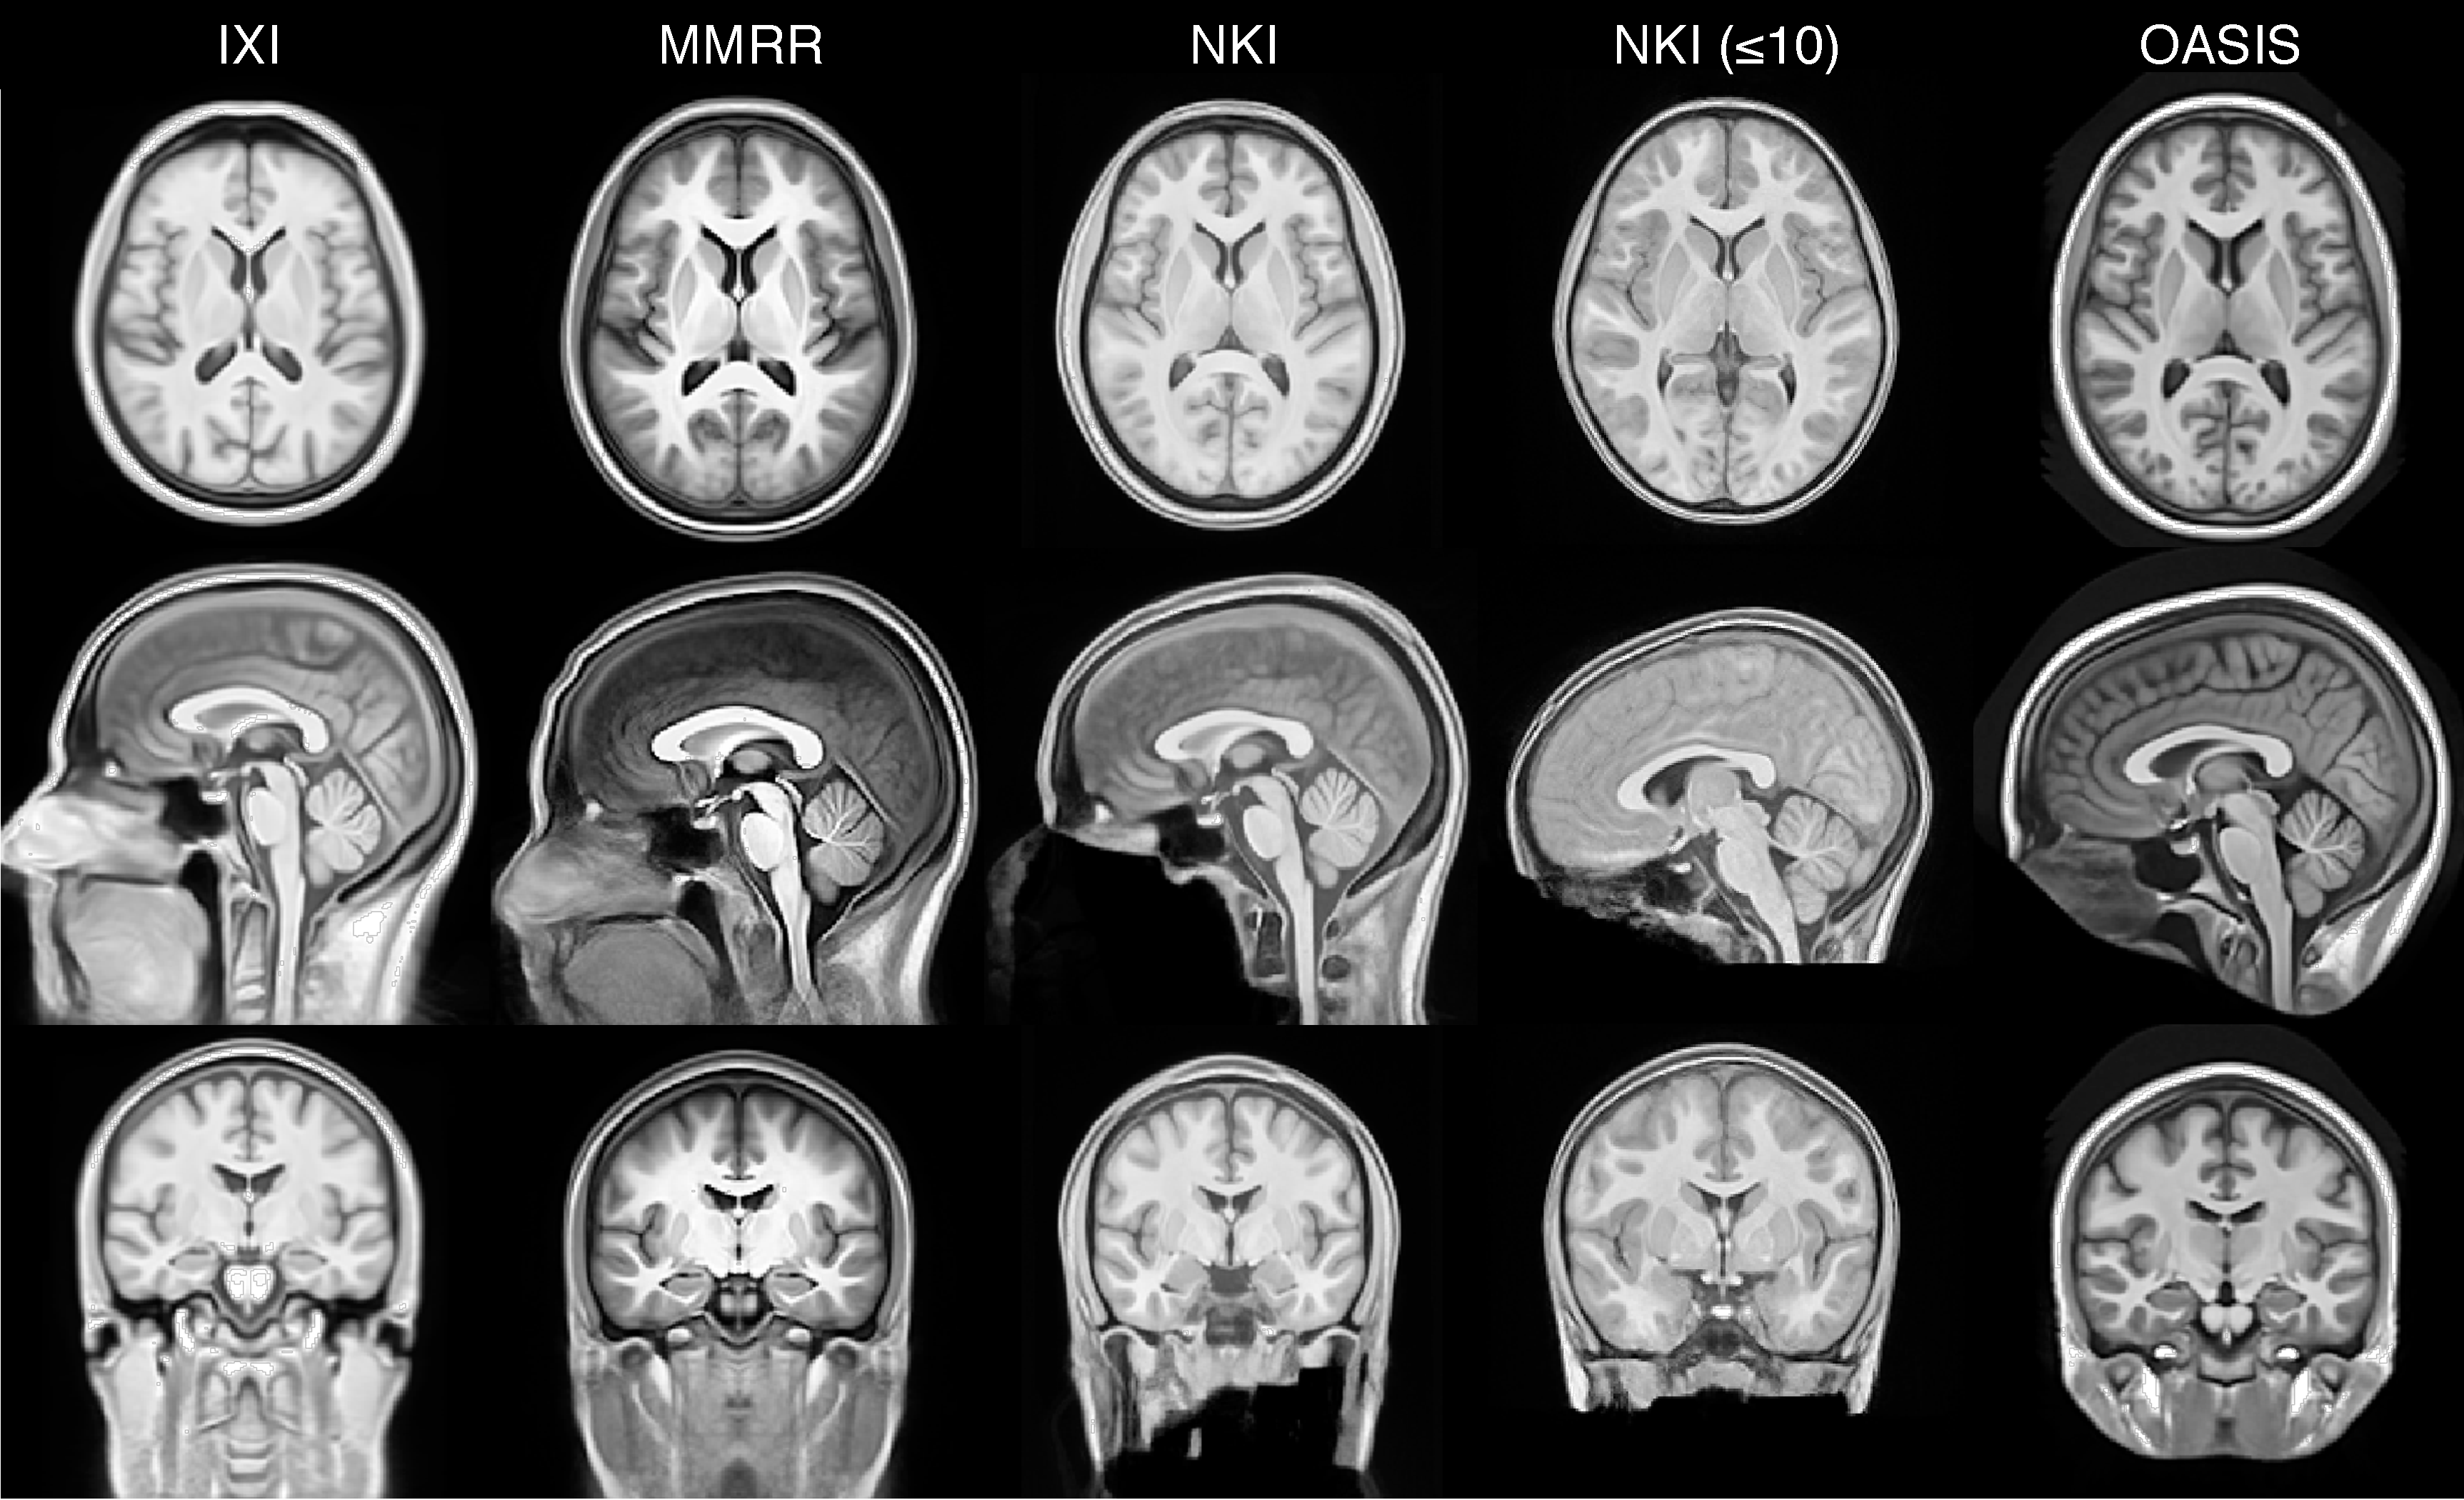
\includegraphics[width=90mm]{Figures/templates.pdf}
  \caption{Population-specific templates for each of the four public data sets used 
  for cortical thickness 
  estimation generated using the script antsMultivariateTemplateConstruction.sh. 
  The benefit of using such templates is obvious considering the variability in
  acquisition and data preparation (e.g. defacing protocols).
  }
  \label{fig:template}
\end{figure}


